\chapter{交流-交流変換}
\label{chap10}

8章で交流から直流を作り，9章で直流から交流を作った。本章で扱うのは最後の組合せ，
交流を別の交流に作り替える\index{こうりゅうこうりゅうへんかん@交流-交流変換}\textbf{交流-交流変換}
（\index{えーしーえーしーへんかん@AC-AC変換}AC-AC変換）である。
実は，このための新しい部品はもう必要ない。8章と9章の回路を直列につなげば，交流から好きな交流が作れるからである。
本章ではまずこの「つなぐだけ」の構成（間接式）が現代の主流であることを確かめ，
そのうえで，直流を介さずに交流を直接作り替える直接式の回路を見ていく。

\begin{screen}
\noindent\textbf{本章の現在地}\\[3pt]
序章の電力変換の地図（\ref{fig0.1}）の最後のマス「交流→交流」に入る。
\textbf{8章の整流回路と9章のインバータを直列につなぐ間接式が現代の主流}であり，
本章はその全体像と，直流を介さない直接式を扱う。
エネルギーの視点で言えば，間接式は\textbf{DCリンクのキャパシタにいったん蓄えてから受け渡す}のに対し，
直接式は\textbf{蓄えずに，スイッチで入力波形を切り出してそのまま受け渡す}。
蓄えないからこそ大きなキャパシタが不要になり，その代わり制御が難しくなる ― この対比が本章の軸である。
\end{screen}

%%======================================================================
\section{交流-交流変換のイメージ}
\label{sec10.1}

\subsection{交流には「大きさ」と「速さ」がある}

直流を特徴づける量は電圧の大きさ1つだけだった。だからDC-DC変換（5〜7章）の仕事は「電圧を変える」ことに尽きた。
これに対して交流は，\index{じっこうち@実効値}\textbf{実効値}（振幅の大きさ）と
\textbf{周波数}（繰り返しの速さ）の2つの量で特徴づけられる。
交流-交流変換とは，この2つを目的に合わせて作り替えることである。
実効値だけを変える変換と，周波数まで変える\index{しゅうはすうへんかん@周波数変換}\textbf{周波数変換}があり，
後者のほうが難しい。本章もこの順に進む。

周波数を変えたい場面の代表はモータの速度制御である。交流モータの回転数は電源周波数にほぼ比例するから，
周波数を自在に変えられれば回転数を自在に変えられる
（\index{かへんそくくどう@可変速駆動}\textbf{可変速駆動}）。
エアコンの圧縮機，電車，ポンプや送風機など，現代のモータ駆動はほとんどこの方式である。
また，東日本（50\,Hz）と西日本（60\,Hz）の電力系統をつなぐ周波数変換所も，
巨大な交流-交流変換器にほかならない。

\subsection{これまでの変換との違い}

これまでの章の変換器は，入力と出力の「形式」を変えるもの（AC-DC，DC-AC）か，
同じ直流どうしで大きさを変えるもの（DC-DC）だった。
交流-交流変換が新しいのは，\textbf{入力も出力も時々刻々変化する波形どうし}を結びつける点である。
このため方式が2つに分かれる。いったん変化しない直流を経由してから作り直す方式と，
変化する入力波形から必要な部分をスイッチで切り出して出力波形を組み立てる方式である。
次節でこの2つを比べる。

%%======================================================================
\section{間接式と直接式の周波数変換}
\label{sec10.2}

\subsection{間接式 ― 8章と9章を直列につなぐ}

\FIGref{fig10.1}の構成を見てほしい。前段は交流を直流に変える整流回路（8章），
後段は直流から任意の周波数・振幅の交流を作るインバータ（9章）であり，
両者の間を\index{でぃーしーりんく@DCリンク}\textbf{DCリンク}と呼ぶ直流部分がつなぐ。
入力の交流はいったん直流になり，そこから改めて交流が作り直される。
どちらの段も既習の回路そのままであり，新しい素子は1つもない。

\begin{figure}[ht]
\begin{center}
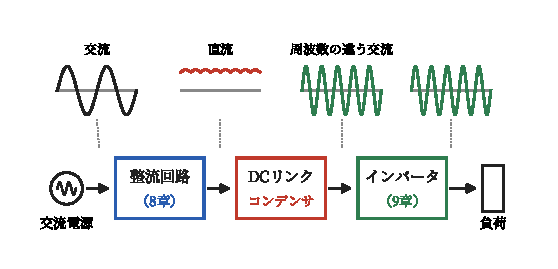
\includegraphics[clip]{figures/fig10.1.eps}
\end{center}
\caption{間接式周波数変換（AC-DC-AC変換）のブロック図。前段は8章の整流回路（実用機では力率改善（PFC）回路を含む），後段は9章のインバータであり，本章で新しく学ぶ素子はない。中間のDCリンクコンデンサがエネルギーの緩衝役を務める}
\label{fig10.1}
\end{figure}

中間に置かれた\index{でぃーしーりんくこんでんさ@DCリンクコンデンサ}\textbf{DCリンクコンデンサ}の役割は，
エネルギーの緩衝である。整流回路の出力は脈打っており（8章），
一方インバータは時々刻々異なる電力を出力側へ送り出す。
入ってくる電力と出ていく電力の瞬時の食い違いを，このキャパシタが充放電で吸収し，DCリンク電圧をほぼ一定に保つ。
4章以来の「エネルギーをいったん蓄えて受け渡す」という考え方が，ここでは変換器2段の間に置かれているのである。

\begin{定義}[間接式と直接式]
\label{def10.1}
交流をいったん直流に変換し，その直流から目的の交流を作り直す方式を
\index{かんせつしきしゅうはすうへんかん@間接式周波数変換}\textbf{間接式周波数変換}
（\index{えーしーでぃーしーえーしーへんかん@AC-DC-AC変換}AC-DC-AC変換）という。
直流を介さず，交流から交流へ直接変換する方式を
\index{ちょくせつしきしゅうはすうへんかん@直接式周波数変換}\textbf{直接式周波数変換}という。
\end{定義}

\subsection{間接式と直接式の長所と短所}

間接式が主流である理由ははっきりしている。
第一に，前段と後段を\textbf{独立に設計・制御できる}。DCリンク電圧さえ一定に保てば，
インバータは入力側の事情を知らなくてよい。
第二に，出力周波数に原理的な制約がなく，入力と無関係に自由な交流を作れる。
第三に，8章・9章の回路として実績と部品の蓄積がそのまま使える。
家庭のインバータエアコンから電車，そして周波数変換所や高電圧直流送電（HVDC）まで，
規模の大小を問わずこの構成が使われている。

代償はDCリンクコンデンサである。
脈打つ電力を吸収するには大きな静電容量が必要で，実機では大型の電解コンデンサが使われることが多い。
変換器の体積の大きな部分を占めるうえ，電解コンデンサは寿命の面でも弱点になりやすい（4章）。
そこで，「\textbf{直流を介さずに済ませば，このコンデンサごと不要になるのではないか}」という発想が生まれる。
これが直接式である。エネルギーを蓄えずに入力から出力へ直接受け渡すため，
理屈のうえでは小型・長寿命にでき，変換が1段で済む分だけ損失も減らせる。
その代わり，時々刻々変化する入力波形から出力を直接組み立てるため制御が難しく，
後で見るように出力周波数や電圧に制約が付く。両者の比較を\TABref{tab10.1}にまとめる。

\begin{table}[ht]
\begin{center}
\caption{間接式と直接式の比較}
\label{tab10.1}
\begin{tabular}{c|c|c}
\hline
& 間接式 & 直接式 \\
\hline
変換の経路 & AC→DC→AC（2段） & AC→AC（1段） \\
エネルギーの緩衝 & DCリンクコンデンサ & なし（直接受け渡す） \\
出力周波数 & 自由 & 方式ごとに制約あり \\
制御 & 各段が独立で容易 & 複雑 \\
主な例 & エアコン・電車・EV & 調光器・大容量モータ \\
\hline
\end{tabular}
\end{center}
\end{table}

\begin{例題}[二段変換の効率]
\label{rei10.1}
間接式変換器で，整流段の効率が$0.95$，インバータ段の効率が$0.95$であるとする。
(a)~全体の効率を求めよ。(b)~出力$5$\,kWのときの内部損失を求めよ。
\begin{解答}
(a) 2段を直列に通るから，全体の効率は積になる。
\begin{equation*}
\eta = 0.95 \times 0.95 \approx 0.90
\end{equation*}
(b) 入力電力は$5/0.90 \approx 5.54$\,kWだから，損失はその差
\begin{equation*}
P_{\mathrm{loss}} = 5.54 - 5 \approx 0.54\,\mathrm{kW}
\end{equation*}
である。段数を重ねるほど効率は積で下がる ― 直接式が1段で変換したくなる理由の1つである。
\end{解答}
\end{例題}

\begin{問}
\item 単相$200$\,V（実効値）の交流を全波整流して平滑した間接式変換器のDCリンク電圧は，
無負荷ではいくらになるか。8章で学んだ「平滑後の電圧はほぼ波形のピーク値」を使って見積もれ。
\end{問}

%%======================================================================
\section{交流位相調整回路}
\label{sec10.3}

\subsection{サイリスタは交流と相性がよい}

直接式の入口として，まず\textbf{実効値だけ}を変える最も簡単な回路から始める。主役は2章のサイリスタである。
サイリスタはゲートにパルスを与えるとオンし（点弧），
いったんオンすると\textbf{ゲートではオフできず}，電流がゼロになるまで流れ続けるのだった（2章のラッチ動作）。
直流回路では「オフできない」ことは欠点だが，交流回路では事情が変わる。
電源電圧が半周期ごとに反転するため，\textbf{電流は半周期ごとに自然にゼロになり，サイリスタは勝手にオフしてくれる}。
これを\index{しぜんてんりゅう@自然転流}\textbf{自然転流}という。
オンのタイミングだけ制御し，オフは電源任せにする ― これがサイリスタ回路の基本方針である。

\begin{figure}[ht]
\begin{center}
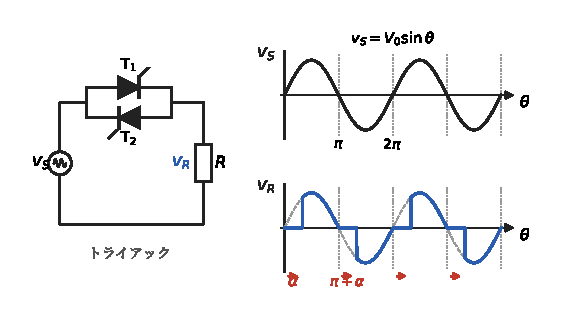
\includegraphics[clip]{figures/fig10.2.eps}
\end{center}
\caption{交流位相調整回路。2個のサイリスタを逆並列にした素子（トライアック）で，各半周期の点弧角$\alpha$以降だけを負荷につなぐ。ゲートパルスは$\theta = \alpha,\ \pi+\alpha,\ 2\pi+\alpha,\ \ldots$で与える}
\label{fig10.2}
\end{figure}

\FIGref{fig10.2}に回路と波形を示す。交流の正負両方の半周期を扱うため，
サイリスタ$\mathrm{T}_1$，$\mathrm{T}_2$を互いに逆向きに並列接続する。
この逆並列対を1素子に集積したものを\index{とらいあっく@トライアック}\textbf{トライアック}という。
各半周期の途中でゲートパルスを与えると，そこから半周期の終わり（電流ゼロ）までが負荷につながり，
電圧波形の前半が削り取られる。
このように交流の位相を基準にオンのタイミングを制御する方式を
\index{いそうせいぎょ@位相制御}\textbf{位相制御}といい，
この回路を\index{こうりゅういそうちょうせいかいろ@交流位相調整回路}\textbf{交流位相調整回路}と呼ぶ。

\begin{定義}[点弧角]
\label{def10.2}
電源電圧のゼロクロス（極性が切り替わる時刻）を基準として，
サイリスタにゲートパルスを与えるまでの位相角$\alpha$を
\index{てんこかく@点弧角}\textbf{点弧角}（位相制御角）という（$0 \le \alpha \le \pi$）。
\end{定義}

\subsection{出力実効値を導く}

負荷（抵抗$R$とする）にかかる電圧の実効値を求めよう。電源電圧を$v_S = V_0 \sin\theta$とすると，
正の半周期では$\alpha \le \theta < \pi$の間だけ$v_R = V_0 \sin\theta$となり，それ以外では$v_R = 0$である。
負の半周期も対称だから，実効値（2乗平均の平方根）は正の半周期$0 \le \theta < \pi$だけで平均して求めてよい。
\begin{equation}
V_{\mathrm{rms}}^2 = \frac{1}{\pi} \int_0^{\pi} v_R^2\, d\theta
= \frac{V_0^2}{\pi} \int_\alpha^{\pi} \sin^2\theta\, d\theta
\label{eq10.1}
\end{equation}
半角の公式$\sin^2\theta = (1-\cos 2\theta)/2$を使って，積分を省略せずに実行する。
\begin{eqnarray}
\int_\alpha^{\pi} \sin^2\theta\, d\theta
&=& \frac{1}{2} \int_\alpha^{\pi} (1 - \cos 2\theta)\, d\theta \nonumber\\
&=& \frac{1}{2} \left[\, \theta - \frac{\sin 2\theta}{2} \,\right]_\alpha^{\pi} \nonumber\\
&=& \frac{1}{2} \left(\pi - \alpha + \frac{\sin 2\alpha}{2}\right)
\label{eq10.2}
\end{eqnarray}
ここで$\sin 2\pi = 0$を使った。式\ref{eq10.2}を式\ref{eq10.1}に戻して平方根を取れば，出力実効値が得られる。
\begin{equation}
V_{\mathrm{rms}} = \frac{V_0}{\sqrt{2}}
\sqrt{1 - \frac{\alpha}{\pi} + \frac{\sin 2\alpha}{2\pi}}
\label{eq10.3}
\end{equation}
検算しておこう。$\alpha = 0$（削らない）なら根号の中は1で，正弦波の実効値$V_0/\sqrt{2}$に戻る。
$\alpha = \pi$（全部削る）なら根号の中は$1 - 1 + 0 = 0$で，出力はゼロになる。
その間の様子を\FIGref{fig10.3}に示す。点弧角を$0$から$\pi$まで動かすだけで，
実効値を最大値からゼロまで連続的に調整できる。

\begin{figure}[ht]
\begin{center}
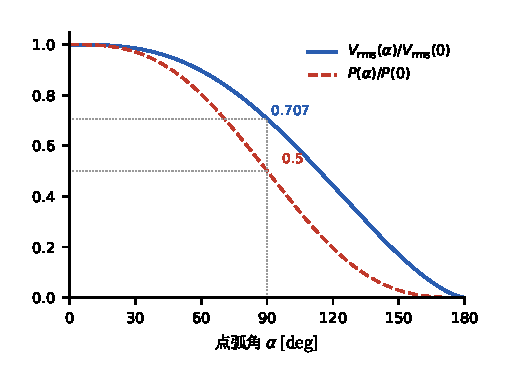
\includegraphics[clip]{figures/fig10.3.eps}
\end{center}
\caption{点弧角$\alpha$と出力実効値・出力電力の関係（式\ref{eq10.3}，抵抗負荷）。$\alpha = 90^\circ$で実効値は$1/\sqrt{2} \approx 0.707$倍，電力はちょうど半分になる}
\label{fig10.3}
\end{figure}

\begin{例題}[位相制御の実効値]
\label{rei10.2}
実効値$100$\,Vの商用電源に交流位相調整回路を挿入し，点弧角を$\alpha = \pi/2$（$90^\circ$）とした。
抵抗負荷にかかる電圧の実効値と，負荷電力が$\alpha = 0$のときの何倍になるかを求めよ。
\begin{解答}
$\sin 2\alpha = \sin \pi = 0$だから，式\ref{eq10.3}の根号の中は$1 - 1/2 + 0 = 1/2$である。
電源の実効値は$V_0/\sqrt{2} = 100$\,Vだから
\begin{equation*}
V_{\mathrm{rms}} = 100 \times \sqrt{\frac{1}{2}} \approx 70.7\,\mathrm{V}
\end{equation*}
となる。抵抗負荷の電力は$P = V_{\mathrm{rms}}^2/R$なので，
$\alpha = 0$のときに対する比は根号の中身そのもの，すなわち$1/2$である。
半周期の半分だけつなぐと電力はちょうど半分 ― 直感どおりの結果になる。
\end{解答}
\end{例題}

この回路は白熱電球の\index{ちょうこうき@調光器}\textbf{調光器}や電気毛布・ヘアドライヤーの熱量調整など，
身近な製品で広く使われてきた。トライアック1個とゲート回路だけで済む簡便さが持ち味である。
7章のリニアレギュレータのように余分な電圧を熱に変えるのではなく，
使わない期間は単に「つながない」だけなので，理想的には損失なしで実効値を調整できる。

\begin{注意}
交流位相調整回路が変えられるのは\textbf{実効値だけ}であり，出力の周波数は入力と同じままである。
また，出力波形は\ref{fig10.2}のとおり正弦波の一部を切り欠いた形になるため，
入力にはない周波数成分（\index{こうちょうは@高調波}\textbf{高調波}）を多く含む。
これは電源側へ流れ出して他の機器を妨害する電磁ノイズの一種であり，11章で正面から扱う。
\end{注意}

\begin{問}
\item 式\ref{eq10.3}の右辺の単位がV（ボルト）になることを確かめよ。
位相角$\alpha$の単位ラジアンが無次元であることに注意せよ。
\item 点弧角を$\alpha = \pi/4$および$\alpha = 3\pi/4$としたとき，
出力実効値は$\alpha = 0$のときの何倍か。また抵抗負荷の電力はそれぞれ何倍か。
\end{問}

%%======================================================================
\section{サイクロコンバータとマトリックスコンバータ}
\label{sec10.4}

\subsection{サイクロコンバータ ― 点弧角を揺らして低周波を描く}

いよいよ直接式で\textbf{周波数}を変える。出発点は8章の三相全波整流回路である。
三相の線間電圧は$60^\circ$（$\pi/3$）ごとに最大の相が入れ替わり，
ダイオードブリッジはその最大値を自動的に乗り継いで直流を作るのだった。
このダイオードをすべてサイリスタに置き換えると，乗り継ぎのタイミングを点弧角$\alpha$だけ遅らせることができ，
出力電圧の平均値を制御できるようになる。線間電圧の振幅を$V_0$とすると，平均出力は
\begin{equation}
\bar{V}_{\mathrm{out}} = \frac{3}{\pi} V_0 \cos\alpha
\label{eq10.4}
\end{equation}
となる（導出は章末問題\ref{ex10.3}）。$\alpha = 0$で最大値$0.955 V_0$，
$\alpha = 90^\circ$でゼロ，さらに$\alpha > 90^\circ$では\textbf{負}になる。
つまり点弧角1つで，出力の平均電圧を正から負まで自在に動かせるのである。

ならば，$\alpha$を時間とともにゆっくり揺らせばどうなるか。
平均電圧が正弦波状に上下し，入力より低い周波数の交流が「平均値として」描かれる（\FIGref{fig10.4}）。
これが\index{さいくろこんばーた@サイクロコンバータ}\textbf{サイクロコンバータ}である。
サイリスタブリッジは電流を一方向にしか流せないため，
実際には正の電流を受け持つ\index{せいぐんぶりっじ@正群ブリッジ}\textbf{正群ブリッジ}と
負の電流を受け持つ\index{ふぐんぶりっじ@負群ブリッジ}\textbf{負群ブリッジ}を逆並列に置き，
出力電流の向きに応じて切り替える。

\begin{figure}[ht]
\begin{center}
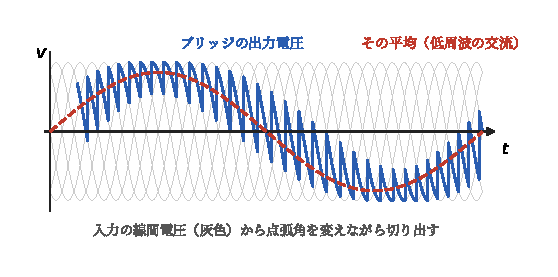
\includegraphics[clip]{figures/fig10.4.eps}
\end{center}
\caption{サイクロコンバータの出力合成のイメージ。三相の線間電圧（灰色）から点弧角を変えながら区分的に切り出すと（青），その平均（赤破線）が入力より低い周波数の正弦波を描く。図は正群ブリッジによる合成を示す}
\label{fig10.4}
\end{figure}

出力波形を入力の乗り継ぎで組み立てる以上，出力の1周期には十分な数の「乗り継ぎ区間」が必要である。
このため出力周波数は入力の$1/3$程度が上限になる。
低速に限られる代わりに，サイリスタの大電流・高耐圧（2章）をそのまま活かせるため，
圧延機や船舶推進など数十MW級の低速・大トルクのモータ駆動で使われてきた。

\subsection{マトリックスコンバータ ― 双方向スイッチのPWM}

出力周波数の制約を取り払うには，サイリスタの自然転流に頼らず，
自分でオン・オフできるスイッチ（IGBTなど）で入力波形を細かく刻めばよい。
ただし交流では電圧も電流も両方向になるため，スイッチには\textbf{双方向}の性能が要る。
\FIGref{fig10.5}のように，IGBT2個とダイオード2個を組み合わせた
\index{そうほうこうすいっち@双方向スイッチ}\textbf{双方向スイッチ}を，
3相入力と3相出力の交点に$3 \times 3 = 9$個並べる。
この行列（マトリックス）状の配置から，
\index{まとりっくすこんばーた@マトリックスコンバータ}\textbf{マトリックスコンバータ}と呼ばれる。

\begin{figure}[ht]
\begin{center}
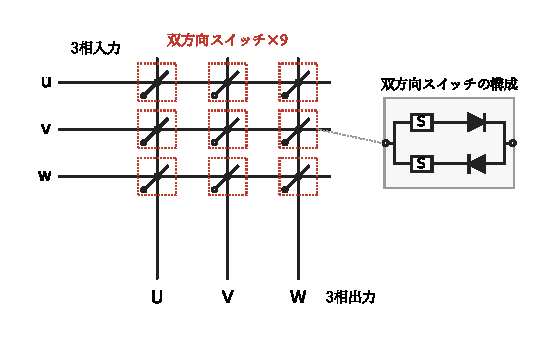
\includegraphics[clip]{figures/fig10.5.eps}
\end{center}
\caption{マトリックスコンバータの構成。3相入力と3相出力のすべての交点に双方向スイッチを置き，どの瞬間に「どの入力相をどの出力相につなぐか」をPWMで選ぶ。右は双方向スイッチの内部構成の例（スイッチとダイオードの逆直列対を逆並列にする）}
\label{fig10.5}
\end{figure}

各出力相は，9章のPWMと同じ考え方で「どの瞬間にどの入力相につなぐか」を高速に切り替え，
パルス幅の平均として目的の正弦波を作る。9章との違いは，刻む対象が一定の直流ではなく，
時々刻々変化する三相の交流だという点だけである。
スイッチングを速くできるので出力周波数は入力より高くもでき，
入力電流も正弦波に近づけられて力率がよい。
DCリンクコンデンサが不要なため小型・長寿命にできる可能性を持ち，理想的な直接式といえる。

\begin{注意}
よいことずくめに見えるマトリックスコンバータが主流になっていないのには理由がある。
第一に制御が複雑である。9個のスイッチは，入力相間の短絡も出力電流の遮断も起こさないよう，
厳密な手順で切り替えなければならない（転流の問題）。
第二に，出力電圧の実効値は原理的に入力の$\sqrt{3}/2 \approx 0.87$倍までしか取れない。
エネルギーの蓄えを持たず，どの瞬間も入力波形の範囲内でしか出力を作れないことの代償である。
現在は航空機など一部の用途で使われ，研究開発が続いている。
\end{注意}

\begin{問}
\item 3相入力・3相出力の変換器を作るとき，サイクロコンバータ（各出力相に正群・負群の三相ブリッジを置く）に必要なサイリスタの個数と，マトリックスコンバータに必要なIGBTの個数（双方向スイッチ1個にIGBT2個を使う）をそれぞれ数えよ。
\end{問}

これで序章の電力変換の地図がすべて埋まった。
直流・交流のあらゆる組合せの変換が，「スイッチで波形を切り出し，インダクタとキャパシタでエネルギーを蓄えて受け渡す」
という同じ原理の組合せで実現できることを見てきた。
残る課題は，高速なスイッチングが必ずまき散らす電磁ノイズである。最終章でこの問題に向き合う。

%%======================================================================
\begin{章末問題}
\item \label{ex10.1}実効値$100$\,Vの電源にトライアック調光器と白熱電球（抵抗負荷とみなす）をつなぐ。
点弧角$\alpha = 60^\circ$，$90^\circ$，$120^\circ$のそれぞれについて，
負荷電圧の実効値と，電力が$\alpha = 0$のときの何倍になるかを求めよ。

\item \label{ex10.2}サイリスタ1個だけの位相制御回路（\ref{fig10.2}で$\mathrm{T}_2$を取り除いた回路）では，
正の半周期の$\alpha \le \theta < \pi$だけが負荷につながり，負の半周期は全く導通しない。
このときの出力実効値が
\begin{equation*}
V_{\mathrm{rms}} = \frac{V_0}{2}
\sqrt{1 - \frac{\alpha}{\pi} + \frac{\sin 2\alpha}{2\pi}}
\end{equation*}
となることを，式\ref{eq10.1}〜式\ref{eq10.3}と同じ手順で導け（この回路では平均を全周期$2\pi$で取ることに注意）。
また，この結果がトライアック版（式\ref{eq10.3}）の$1/\sqrt{2}$倍である理由をエネルギーの言葉で説明せよ。

\item \label{ex10.3}三相サイリスタブリッジの出力は，点弧角$\alpha$のとき
$\theta = \pi/3 + \alpha$から$2\pi/3 + \alpha$までの区間で$V_0 \sin\theta$となる（$V_0$：線間電圧の振幅）。
この区間の平均値を積分で計算し，式\ref{eq10.4}を導け。
また$\alpha = 0^\circ$，$60^\circ$，$90^\circ$，$120^\circ$のときの平均出力を$V_0$を単位として求めよ。

\item \label{ex10.4}出力$10$\,kWのモータ駆動を，(i)~間接式（整流段の効率$0.96$，インバータ段の効率$0.96$）と，
(ii)~マトリックスコンバータ（効率$0.96$）で行う場合とで比べる。
\begin{enumerate}
\item[(a)] それぞれの全体効率を求めよ。
\item[(b)] それぞれの内部損失を求め，比較せよ。
\item[(c)] 損失で不利にもかかわらず間接式が主流である理由を，本章の内容から2つ挙げよ。
\end{enumerate}
\end{章末問題}
